% 
% Annual Cognitive Science Conference
% Sample LaTeX Paper -- Proceedings Format
% 

% Original : Ashwin Ram (ashwin@cc.gatech.edu)       04/01/1994
% Modified : Johanna Moore (jmoore@cs.pitt.edu)      03/17/1995
% Modified : David Noelle (noelle@ucsd.edu)          03/15/1996
% Modified : Pat Langley (langley@cs.stanford.edu)   01/26/1997
% Latex2e corrections by Ramin Charles Nakisa        01/28/1997 
% Modified : Tina Eliassi-Rad (eliassi@cs.wisc.edu)  01/31/1998
% Modified : Trisha Yannuzzi (trisha@ircs.upenn.edu) 12/28/1999 (in process)
% Modified : Mary Ellen Foster (M.E.Foster@ed.ac.uk) 12/11/2000
% Modified : Ken Forbus                              01/23/2004
% Modified : Eli M. Silk (esilk@pitt.edu)            05/24/2005
% Modified : Niels Taatgen (taatgen@cmu.edu)         10/24/2006
% Modified : David Noelle (dnoelle@ucmerced.edu)     11/19/2014
% Modified : Roger Levy (rplevy@mit.edu)     12/31/2018



%% Change "letterpaper" in the following line to "a4paper" if you must.

\documentclass[10pt,letterpaper]{article}

\usepackage{cogsci}
\usepackage{pslatex}
\usepackage{apacite}
\usepackage{float} % Roger Levy added this and changed figure/table
                   % placement to [H] for conformity to Word template,
                   % though floating tables and figures to top is
                   % still generally recommended!
\usepackage{booktabs}
                   
%\cogscifinalcopy % Uncomment this line for the final submission 


%\usepackage[none]{hyphenat} % Sometimes it can be useful to turn off
%hyphenation for purposes such as spell checking of the resulting
%PDF.  Uncomment this block to turn off hyphenation.

\usepackage{graphicx}
\usepackage{amsmath}
\usepackage{xcolor}
\usepackage{url}
% \usepackage{hyperref}
% \hypersetup{
%     colorlinks,
%     urlcolor={blue!80!black}
% }

\newcommand{\tableref}[1]{Table~\ref{#1}}
\newcommand{\figref}[1]{Figure~\ref{#1}}
\newcommand{\expref}[1]{Exp.~#1}

%\setlength\titlebox{4.5cm}
% You can expand the titlebox if you need extra space
% to show all the authors. Please do not make the titlebox
% smaller than 4.5cm (the original size).
%%If you do, we reserve the right to require you to change it back in
%%the camera-ready version, which could interfere with the timely
%%appearance of your paper in the Proceedings.

\definecolor{Red}{RGB}{180,20,140}
\definecolor{Blue}{RGB}{0,0,255}
\newcommand{\jd}[1]{\textcolor{Red}{\textbf{[jd: #1]}}} 
\newcommand{\lk}[1]{\textcolor{Blue}{\textbf{[lk: #1]}}} 

\title{Seeing is believing: testing an explicit linking assumption for visual world eye-tracking in psycholinguistics} 
 
\author{{\large \bf Judith Degen (jdegen@stanford.edu)} \\
  Department of Linguistics, 450 Jane Stanford Way \\
  Stanford, CA 94305 USA
  \AND {\large \bf Leyla Kursat (lkursat@stanford.edu)} \\
  Department of Linguistics, 450 Jane Stanford Way \\
  Stanford, CA 94305 USA
  \AND {\large \bf Daisy Leigh (ddleigh@stanford.edu)} \\
  Department of Linguistics, 450 Jane Stanford Way \\
  Stanford, CA 94305 USA}


\begin{document}

\maketitle


\begin{abstract}

\jd{write}

\textbf{Keywords:} 
psycholinguistics; experimental pragmatics;  scalar implicature; linking functions; visual world; eye-tracking
\end{abstract}


\section{Introduction}

Experimental investigation is integral to scientific inquiry in cognitive science, and experimental data has informed cognitive theory-building for centuries. A fundamental ingredient in  using empirical data to put theories to the test is the assumption made by researchers about the mapping between theoretical notions and empirical measurements: the \emph{linking assumption}. Indeed, empirical measurements are only informative if the  linking assumption is (sufficiently) clear and justified. We argue that both clarity and justification are often lacking for linking assumptions made in \emph{visual world eye-tracking}, a widely used experimental method in psycholinguistic research. We highlight the role that visual world eye-tracking has played in the burgeoning field of experimental pragmatics, which suffers particularly acutely from a lack of clear and justified linking assumptions. We then test a (usually implicitly) made linking assumption for referential tasks, which we term the \emph{Referential Belief} linking assumption: that the proportion of looks to a referent in a time window reflects participants' degree of belief that the referent is the intended target in that time window. To do so, we compare eye movement data against explicit beliefs collected in an incremental decision task. We make use of a previously collected eye movement dataset on scalar implicature processing \cite<\expref{3} of>{sun2020}. In \expref{1} we collect explicit beliefs to test against \citeA{sun2020}'s eye movement data. In \expref{2}, we replicate  \citeA{sun2020} in a web-based eye-tracking paradigm using \texttt{WebGazer.js}. 

\section{Linking assumptions for visual world eye-tracking}

Visual world eye-tracking (VWE) is a widely used measure in psycholinguistics, fruitfully driving advances in our understanding of phonetic, lexical, syntactic, prosodic, semantic, and pragmatic processing  \cite{tanenhaus1995,Allopenna1998,altmann1999,clayards2008,SedivyEtAl1999:Achieving-Incremental-Semantic-,huang2009,kurumada2014}. %LeffelXiangKennedy2016:Imprecision-is-Pragmatic-,}
In standard VWE tasks, participants view displays of objects while listening to spoken sentences while their eye movements are monitored (see \figref{fig:display} for an example). The popularity of VWE stems from one of its very desirable features: eye movements can be interpreted as an indicator of attention that is closely time-locked to the linguistic signal and not subject to voluntary control \jd{get ref for this}. Language can guide eye movements to a region of interest in a display within 200 ms \cite{Allopenna1998}. By sampling an x/y coordinate every few milliseconds, researchers thus obtain a very temporally fine-grained record of participants' language-directed attention over the course of an unfolding utterance. This property has been particularly useful in resolving questions regarding the time-course of online language processing, which typically cannot be addressed using offline measures like forced choice, truth-value judgments, or even more coarse-grained temporal measures like response times from button presses. Notable VWE findings that could not have been obtained with more coarse-grained measures include the diverse insights that visual context is rapidly integrated into syntactic structure assignment \cite{tanenhaus1995,chambers2004}, that words are processed incrementally and listeners maintain uncertainty about past input \cite{Allopenna1998,clayards2008}, and that listeners anticipate upcoming linguistic material based on selectional restrictions and rapid pragmatic reasoning \cite{altmann1999,SedivyEtAl1999:Achieving-Incremental-Semantic-}.

These notable successes notwithstanding, there is an elephant in the room: we still have a relatively poor understanding of how to link observed eye movements to the underlying mental processes that generate them \cite{SalverdaTanenhaus2017:The-Visual-World-Paradigm, tanenhaus2000eye, Allopenna1998, magnuson2019fixations}. The problem of interpretability  is compounded by the fact that VWE is used in vastly different tasks. Consider just the difference between active referential tasks (in which participants' goal is to identify and select the speaker's intended referent) and passive predictive tasks (in which participants simply watch a display while listening to language, without an overt task or goal). In the former case, arguments are made that eye movements reflect listeners' active search for or belief in the referent, depending on whether visual information about the display has been integrated. In the latter case, the evidence indicates that eye movements reflect an automatic predictive process \cite{altmann1999}. But what, exactly, does this mean? What is the generative process by which, e.g., a notion like ``prediction" ultimately results in an eye movement to a region at a particular point in time? Few make clear assumptions about the generative process underlying eye movements \cite<but for a principled early example, see >{Allopenna1998}.

Here, we test an explicit linking assumption for referential tasks, which we term the Referential Belief linking assumption: that the proportion of looks to a referent in a time window reflects participants' degree of belief that the referent is the intended target in that time window. This linking assumption was tested and found not supported in previous work \cite{QingLD2018}. In a re-analysis of an experimental semantics dataset on the processing of relative and absolute gradable adjectives \cite{LeffelXiangKennedy2016:Imprecision-is-Pragmatic-}, \citeA{QingLD2018} found that explicit beliefs collected in an incremental decision task \cite<similar to gating tasks,>{Allopenna1998} did not correlate with eye movements, with the exception of one condition. They argued that the reason for the lack of support may have been participants' close to zero expectation  for observing the linguistic stimuli used in the original experiment, where expectation was linked to production probabilities elicited in a separate free production task.

Of course, it is also possible that the incremental decision task simply does not capture the beliefs that inform eye movements. We believe this is unlikely, given recent successes in using such tasks to elicit contrastive inferences \cite{KreissDegen2020, alsop2018}, but acknowledge the possibility. The previous failure to find support for the Referential Belief link, compounded by the concern regarding the validity of the incremental decision task, motivates the current study: to test the Referential Belief link on a different dataset. For this purpose, we replicate \expref{3} of \citeA{sun2020} (henceforth, ``SB2020") in an incremental decision task rather than an eye-tracking task (\expref{1}) and ask how well the explicit beliefs predict the eye movement data. \jd{webgazer?}


\section{Test bed: Sun \& Breheny (2020)}

We replicate \expref{3} of SB2020, which addressed a now classic question in experimental pragmatics: is the processing of scalar inferences delayed relative to the processing of literal information \cite{bott2004, Breheny2006, huang2009, grodner2010, DegenTanenhaus2015, DegenT2016, Tomlinson2013}? In particular, SB2020 were interested in assessing the possible effect of two factors on the speed with which determiners are processed: first, pre-existing low-level associations between determiners and set sizes (i.e., a preference for \emph{all} to be associated with bigger set sizes and for \emph{some} to not show a clear preference, as established in a norming study); and second, whether the application of the determiner to a set of objects can be verified without checking a separate set of objects. For instance, the partial utterance \emph{Click on the boy that has three}, heard in the left display of \figref{fig:display}, requires only verifying that there is a boy with three objects. In contrast, replacing \emph{three} with either \emph{all} or \emph{some} requires additionally verifying that there are no other apples in the display or -- if \emph{some} is pragmatically enriched to \emph{not all} --  that there is at least one other orange in the display, respectively. That is, \emph{all} and \emph{some} should require additional processing time before settling on the target, but if \emph{some} is immediately enriched to \emph{some, but not all}, verification looks to what SB2020 call the `residue set' (the remaining objects in the center of the screen) should increase immediately after observing the determiner. 

\begin{figure}[H]
\centering
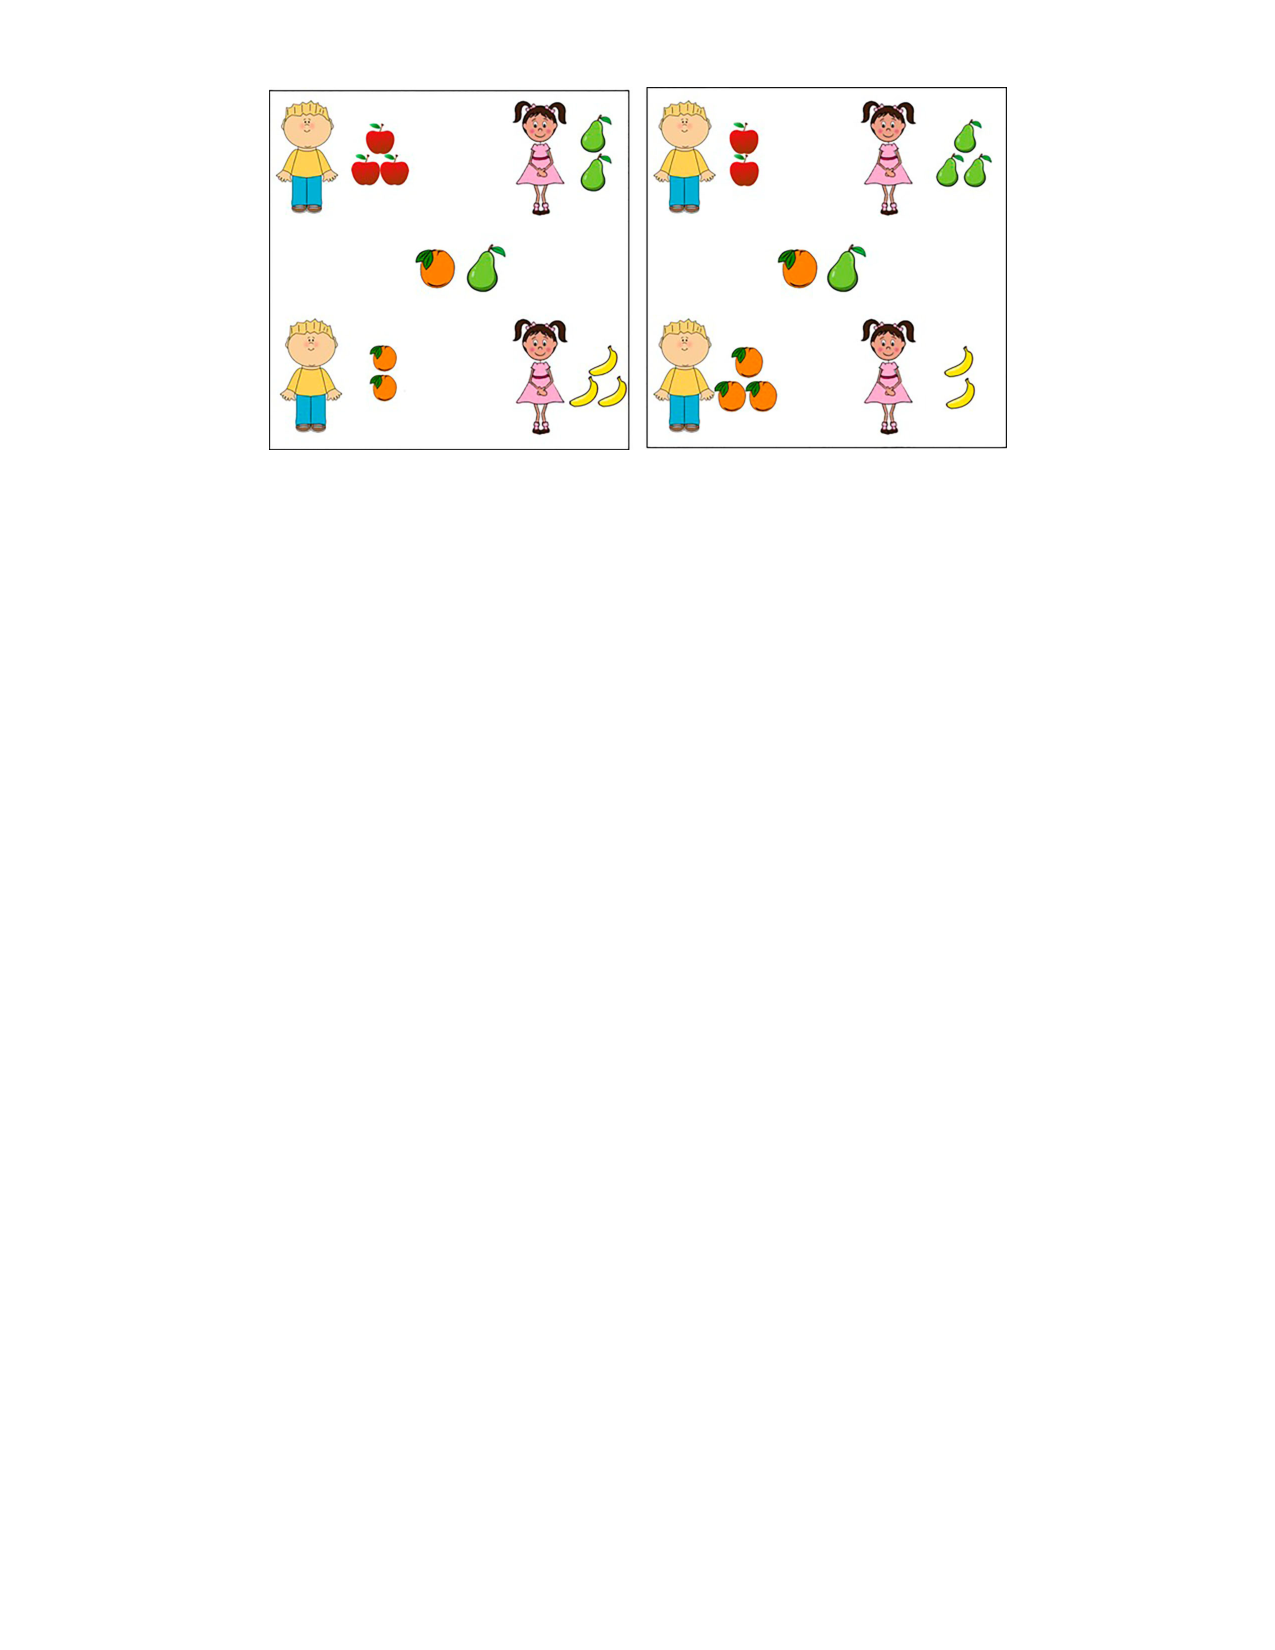
\includegraphics[width=\columnwidth]{images/display}
\caption{Example displays from \expref{3} of SB2020. The left image (big \emph{all}/ small  \emph{some}) was paired with  \emph{Click on the boy that has all/three of Susan's apples} or  \emph{Click on the girl that has some/two of Susan's pears}. The right image (small  \emph{all}/ big  \emph{some}) was paired with  \emph{Click on the boy that has all/two of Susan's apples} or  \emph{Click on the girl that has some/three of Susan's pears}.} 
\label{fig:display}
\end{figure}

Their predictions were borne out (see proportions of looks in  \figref{fig:results-original}, top). In the determiner window (200ms after determiner onset to 200ms after name onset) and the name window (200ms after name onset to 200ms after noun onset), number terms led to more (and a faster increase in) target looks than did \emph{all} and \emph{some}, suggesting that the need for verification of the residue set is a source of relatively fewer target looks for \emph{all} and \emph{some}. Moreover, while there was no effect of set size in the number or \emph{some} condition, big \emph{all} led to more target looks than small \emph{all}. Finally, and crucially for their purposes, they found that looks to the residue set in the determiner window increased for both \emph{all} and \emph{some} (but not numbers) equally and at the same time. 



Jointly, their results support what they call the fast-pragmatic account: the view that the computation of scalar inferences itself is not delayed compared to literal processing, and that previously reported apparent slowdowns in processing of \emph{some} are instead likely due to joint effects of verification time and low-level set size associations for \emph{all} which facilitate the processing of big \emph{all} compared to small \emph{some}. 

\begin{figure}[tbh!]
\centering
%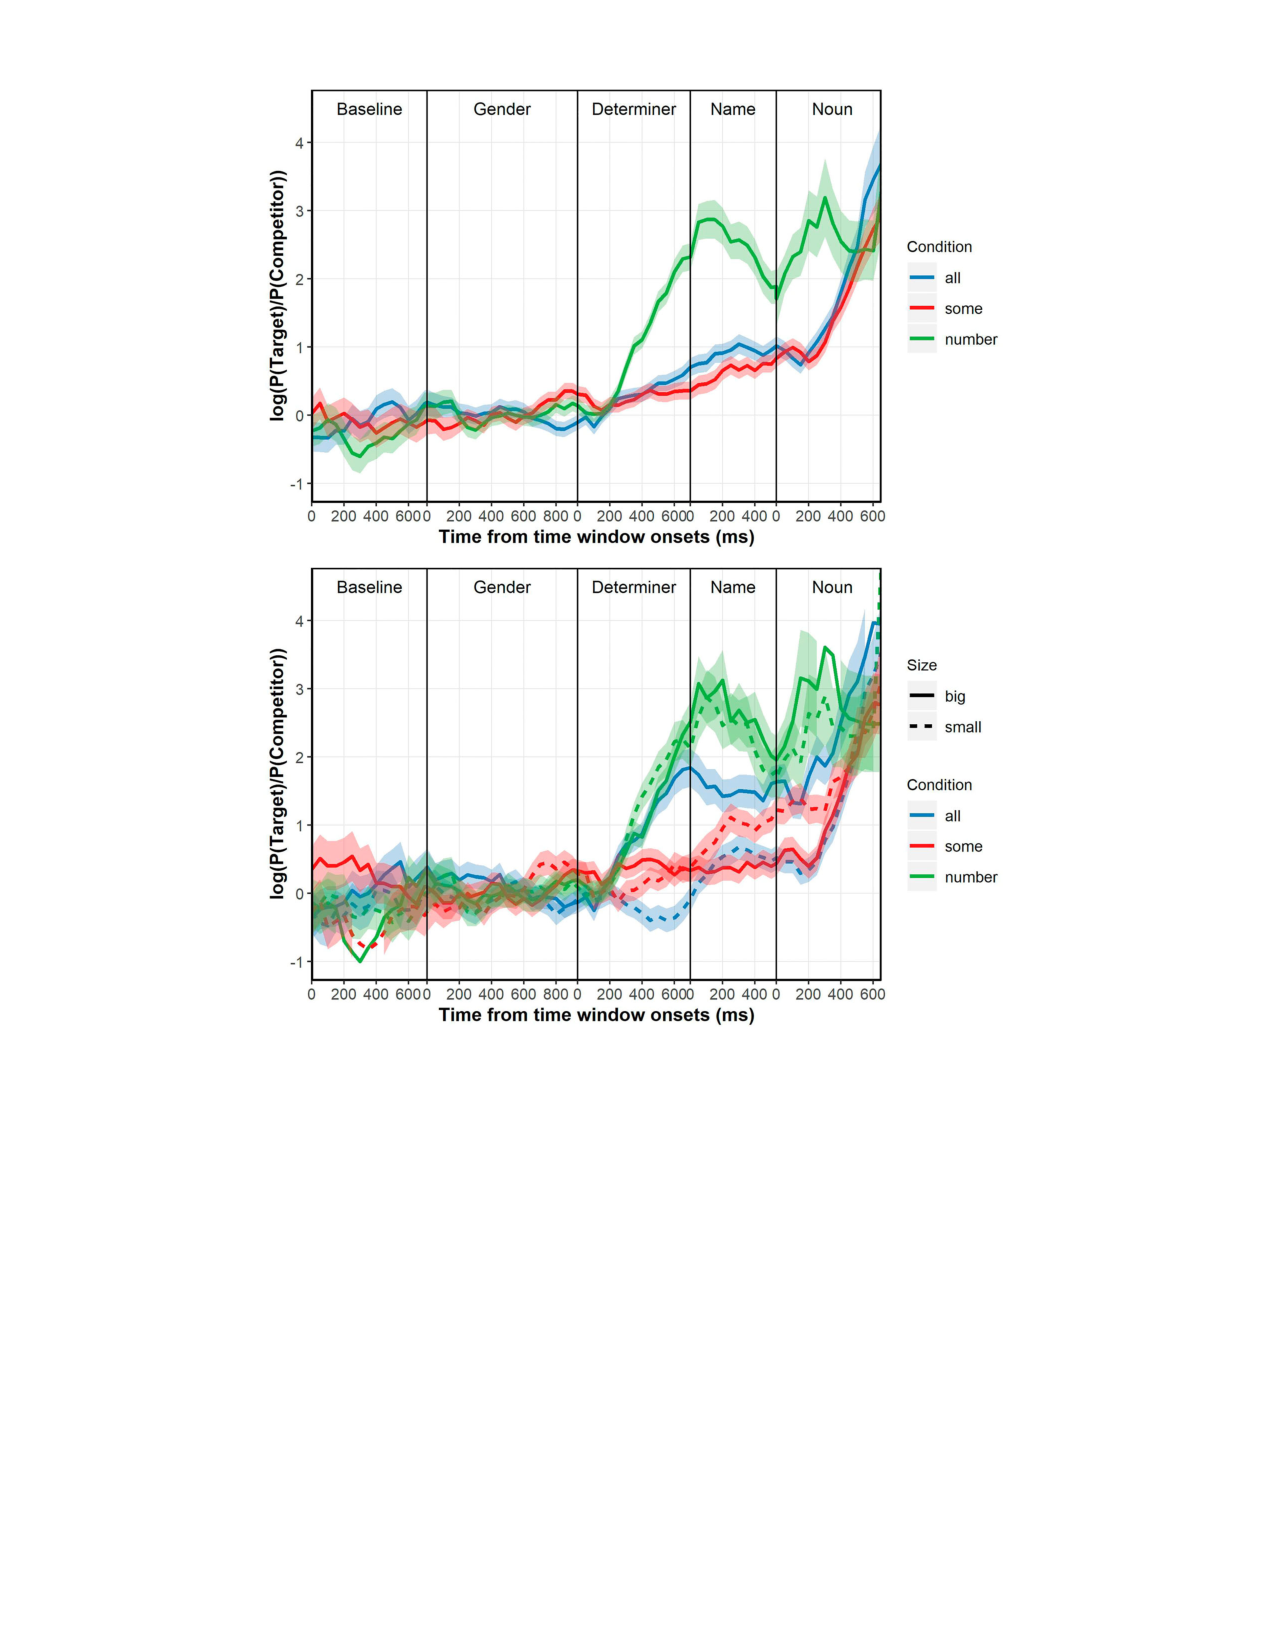
\includegraphics[width=\columnwidth]{images/results-original}
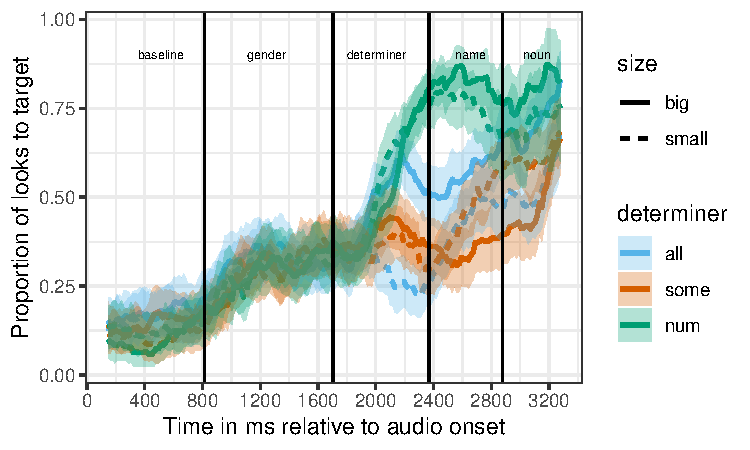
\includegraphics[width=\columnwidth]{../../analysis/SunBreheny/1_incremental/main/graphs/proportions_condsize_withresidue_target}
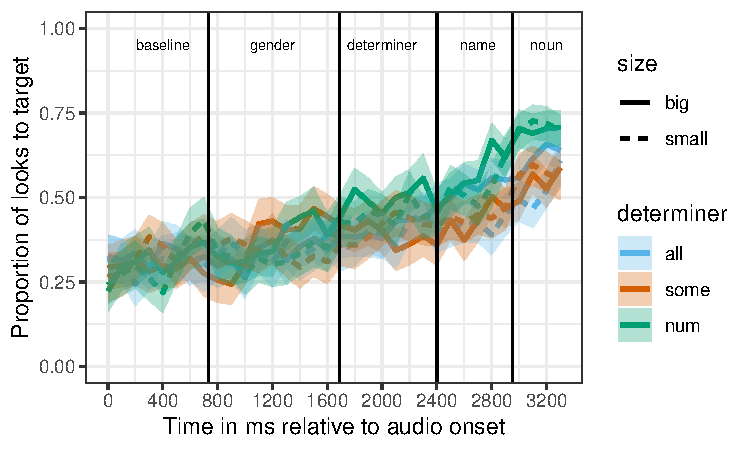
\includegraphics[width=\columnwidth]{../../analysis/SunBreheny/2_webgazer/main/graphs/proportions_condsize_withresidue_target}
\caption{Proportion of target looks (out of target, competitor, and residue looks) from instruction onset. Transparent ribbons indicate 95\% bootstrapped confidence intervals. Black vertical lines indicate onsets of analysis windows of interest (window labels at top of graphs). \textbf{Top:} \expref{3} of SB2020. \textbf{Bottom:} Our \expref{2}.}
\label{fig:results-original}
\end{figure}

\begin{figure}[tbh!]
\centering
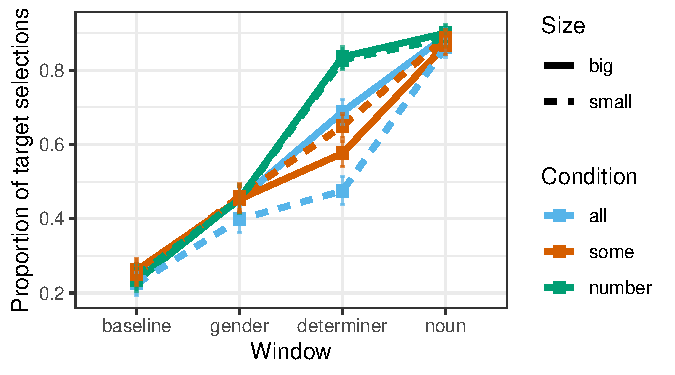
\includegraphics[width=\columnwidth]{../../analysis/SunBreheny/1_incremental/main/graphs/results-target-all-looks}
%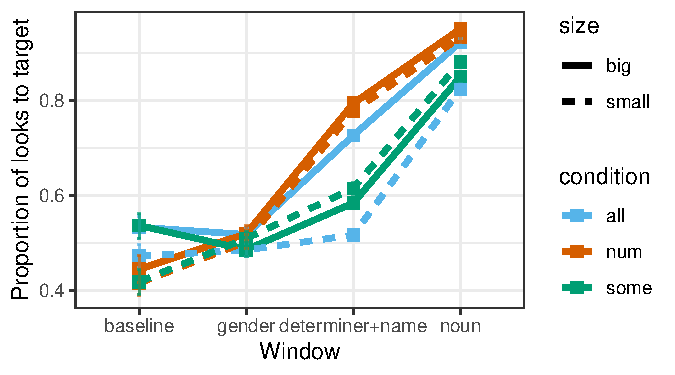
\includegraphics[width=\columnwidth]{../../analysis/SunBreheny/1_incremental/main/graphs/results-target}
%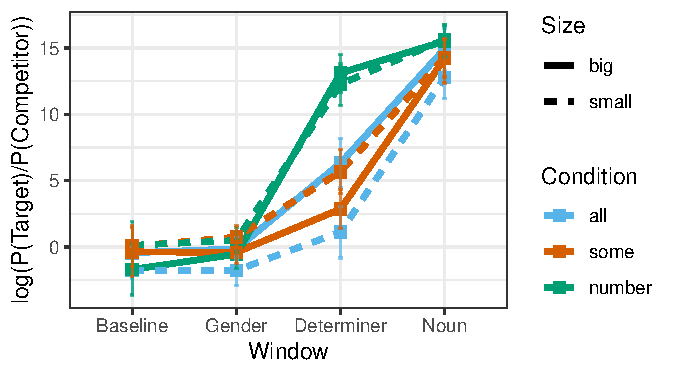
\includegraphics[width=\columnwidth]{../../analysis/SunBreheny/1_incremental/main/graphs/results-idt}
\caption{Proportion of target selections in \expref{1} by quantifier and set size. Error bars indicate 95\% bootstrapped confidence intervals.} 
\label{fig:results-idt}
\end{figure}


For the purpose of testing the Referential Belief linking assumption, this study has both appealing features as well as one glaring problem. The appealing features include the simple 2x3 design, a limited and clearly defined set of referents in each display, and the clarity of the referential task. The glaring problem, which disqualifies the Referential Belief link as a full linking theory from the outset, are the systematic looks to the residue set: the Referential Belief link is only defined for looks to possible referents. There is no plausible argument to be made that participants look to the residue set because they believe it may be the intended target.  Thus, we have already identified one way in which, if otherwise supported by the data, the Referential Belief link will have to be extended. We return to this point in the General Discussion.


\section{Exp.~1: replicating Sun \& Breheny (2020) using an incremental decision task}

In order to measure participants' beliefs about the intended referent at points in the utterance that would allow us to compare explicit beliefs to proportions of looks in SB2020, participants engaged in an incremental decision task \cite{Allopenna1998,QingLD2018, KreissDegen2020,alsop2018}. 

\subsection{Methods}

\textbf{Participants.} We recruited 120 participants on Mechanical Turk, excluding participants with $<$ 95\% accuracy (n=29) and trials on which participants selected the wrong referent in the last window (665 trials). All participants were self-reported native English speakers.\footnote{Procedure, materials, analyses and exclusions were pre-registered at \url{https://rb.gy/ecoggz} (Exp.~1) and \linebreak \url{https://rb.gy/ednwye} (Exp.~2). The collected sample size for Exp.~2 (183 participants) was larger than the originally pre-registered sample size (102 participants) because 40\% of the initially tested 102 participants had a technical issue and weren't able to see the whole display.}

\textbf{Materials and procedure.} We measured participants' beliefs about the intended referent for each display shown to participants by SB2020 (see \figref{fig:display} for examples). Participants were told that they were playing a guessing game, and whenever they made a guess, more words would appear. The critical sentences of the form ``Click on the GENDER who has DETERMINER  of NAME's NOUN" were revealed incrementally. GENDER was one of \emph{boy/girl}, DETERMINER was one of \emph{some/all/two/three}, NAME was one of \emph{Susan/Amy/Michael}, and NOUN was one of \emph{apples/bananas/erasers/scissors/knives/rulers/forks/plates/
spoons/pencils/pears/oranges}.  Participants clicked on the presumed target after (a) ``Click on the" (baseline window), (b) ``GENDER that has" (gender window), (c) ``DETERMINER of NAME's" (determiner window), and (d) ``NOUN" (noun window). After each click, the next word(s) or display was shown. After 6 practice trials, each participant saw 48 experimental trials, of which 12 were filler trials with the number terms \emph{one} and \emph{four}. The 36 critical trials implemented SB2020's 2 (big vs.~small target set) by 3 (\emph{all, some}, number) design. 


\subsection{Results and discussion}

%Following \citeA{sun2020}, we computed the target preference score $\ln (\frac{p(\text{target})}{p(\text{competitor})})$ for each time window, where  $p(\text{target})$ and $p(\text{competitor})$ refer to the proportion of target and competitor selections, respectively (see \figref{fig:results-idt}). Proportions were aggregated by subject, determiner, and set size. 

\figref{fig:results-idt} shows proportions of target selections out of all selections in each time window and condition. 


\textbf{Data analysis}. SB2020 fit separate linear regression models to target advantage scores in time windows of interest. We instead fit logistic mixed effects models predicting target selections. This choice was motivated by logistic regression being the more principled approach to modeling categorical data. It also avoids problems like pre-aggregating data and adding smoothing terms to avoid division by zero or discarding mathematically problematic data points. %\jd{The results are qualitatively identical if we instead run linear models on target preference scores. (??)}

SB2020 fit separate models to the baseline, gender, determiner, name, and noun windows (though only the determiner and name windows were of interest). We collapsed the name window into the determiner window because the name does not add disambiguating information. The models predicted target over competitor choices from fixed effects of quantifier (reference level: ``number"), centered size (higher value: ``big"), by-item and by-subject random intercepts, and random by-subject slopes for condition and size. No effects reached significance in the baseline, gender, and noun window, as expected.\footnote{In fact, fitting models to the noun window was impossible because participants, with very few exceptions, always chose the target. That is, there was no variance to speak of that a model could be estimated to explain.}  In the determiner window, the window of interest, there were main effects of condition, such that target selections were less likely in both the \emph{some} ($\beta$=-2.90, $SE$=0.36, $p<$.0001) and \emph{all} ($\beta$=-2.92, $SE$=0.36, $p<$.0001) conditions, compared to the number condition. There was no main effect of size, consistent with the visual result that target selections in the number condition are not modulated by  target set size ($\beta$=-0.09, $SE$=0.26, $p<$.73). However, we did observe interactions between quantifier and size, such that small sets resulted in more target selections for \emph{some} ($\beta$=0.59, $SE$=0.28, $p<$.05) but fewer target selections for \emph{all} ($\beta$=-1.27, $SE$=0.29, $p<$.0001), compared to number terms. 

%(Intercept)          3.77254    0.39655   9.513  < 2e-16 ***
%conditionall        -2.92409    0.36359  -8.042 8.81e-16 *** 		replicates
%conditionsome       -2.90211    0.36217  -8.013 1.12e-15 ***		replicates
%csize               -0.09207    0.26069  -0.353   0.7239    			does not replicate -- they found main effect (more looks to big set and steeper increase)
%conditionall:csize  -1.27305    0.28523  -4.463 8.08e-06 ***		replicates
%conditionsome:csize  0.59465    0.27945   2.128   0.0333 *  		does not replicate , they found null effect (but perhaps in name window? they don't report this specifically)



\textbf{Comparison with SB2020: replication analysis}. These results constitute a near-perfect replication of  SB2020. Most of their effects reported in the determiner window replicated, with two exceptions (see overview in \tableref{tab:replication}): we did not observe a main effect of set size, while they did; and we observed an interaction of size and determiner such that small \emph{some} led to greater target selections than big \emph{some}. These differences are not as big as they may seem: in our dataset, the lack of set size main effect can be explained by the interactions with determiner: while size makes no difference at all for number (the determiner predictor reference level), it has the opposite effect for \emph{all} compared to \emph{some}. A similar tendency can be observed in SB2020's results when taking into account the joint determiner and name windows. In fact,  SB2020 report the absence of a main effect for size in the name window, and instead an interaction between size and determiner. While they do not report the same post hoc analyses, visual inspection of \figref{fig:results-original} (top) suggests that the interaction in the name window is indeed the result of set size having the opposite effect for \emph{all} compared to \emph{some}. Thus, when taking into account their results from both the determiner and name window, which we collapsed into one, the results are qualitatively identical. The different results reported by  SB2020 in the two time windows are presumably the result of certain information taking longer to be integrated, something which the incremental decision task by its offline nature cannot capture. %\jd{if time, re-analyze their results with logistic models?}

\begin{figure*}
\centering
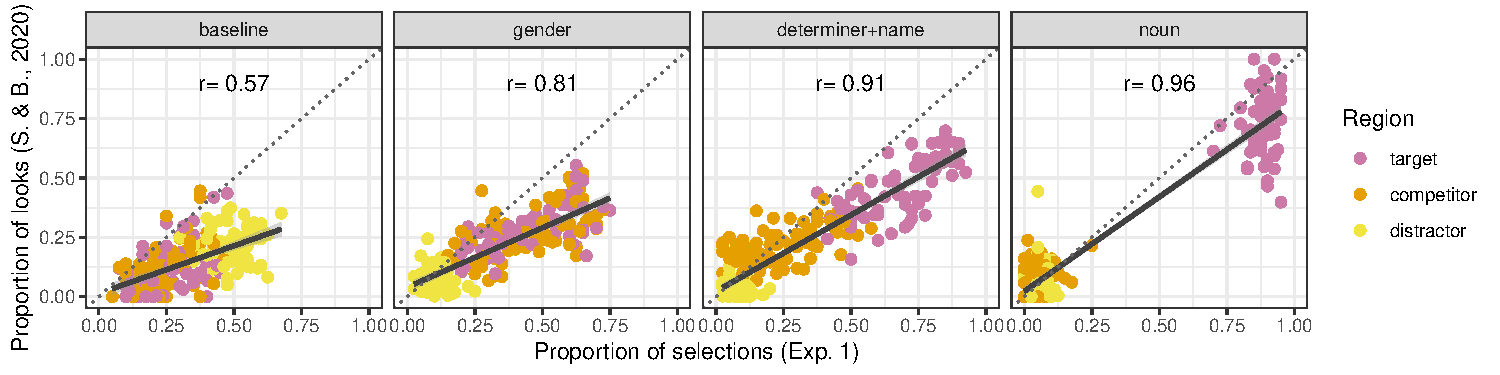
\includegraphics[width=.9\textwidth]{../../analysis/SunBreheny/1_incremental/main/graphs/corr-window}
\caption{Proportions of looks in SB2020 against proportions of selections in \expref{1}. Facets indicate time windows.} 
\label{fig:corr-window}
\end{figure*}

%\begin{figure}
%\centering
%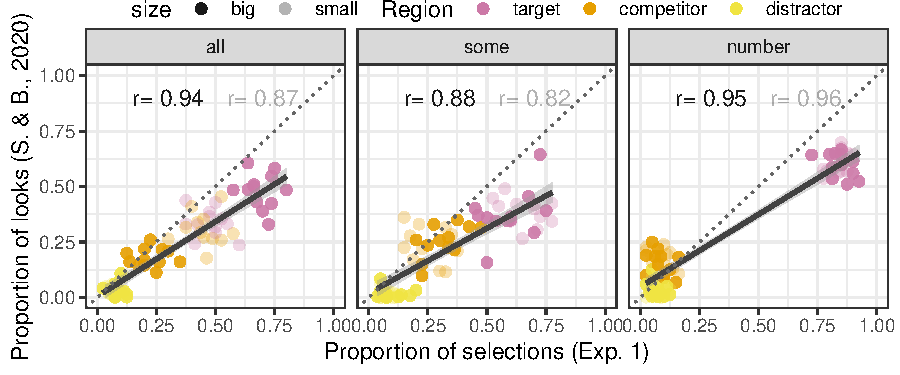
\includegraphics[width=\columnwidth]{../../analysis/SunBreheny/1_incremental/main/graphs/corr-determiner}
%\caption{Proportions of determiner+name window looks in \citeA{sun2020} against proportions of selections in \expref{1}. Facets indicate determiner, dot transparency indicates target set size, color indicates region of interest.\jd{skip this one or add qualitative remark about looks and selections being more extreme for number than others? but that's basically already there in the proportions of target selections plot and is discussed in replication section}} 
%\label{fig:corr-determiner}
%\end{figure}

\begin{figure}
\centering
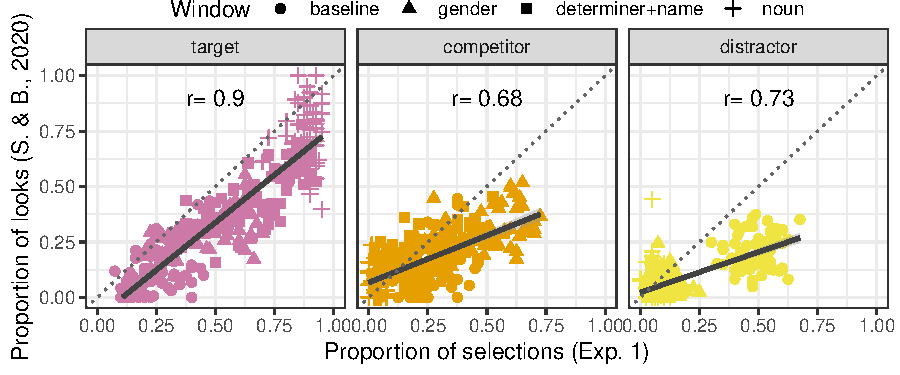
\includegraphics[width=\columnwidth]{../../analysis/SunBreheny/1_incremental/main/graphs/corr-region}
\caption{Proportions of looks in SB2020 against proportions of selections in \expref{1}. Facets indicate region of interest.} 
\label{fig:corr-region}
\end{figure}

\textbf{Comparison with SB2020: linking function analysis}. \figref{fig:corr-window} shows the correlation between  proportion of selections in \expref{1} and proportions of looks in SB2020. The overall correlation was very high ($r(862) = .87$, $p < .0001$), suggesting preliminary support for the Referential Belief link. To investigate whether the predictive power of explicit beliefs was modulated by additional factors, we conducted a linear regression analysis %\footnote{\jd{Beta regression is the appropriate analysis here because prooprtions are bounded by [0,1]. For simplicity, linear regression. If time, also do Beta regression and report whether results similar.}} 
predicting proportion of looks from fixed effects of proportion of selections (mean-centered) and its 2-way interactions with time window (dummy-coded, reference level: `determiner') and region of interest (dummy-coded, reference level: `target'). There was a large and significant effect of selection proportion  ($\beta$=0.79, $SE$=0.02, $t$=32.31, $p<$.0001), such that stronger beliefs resulted in more looks. This effect was modulated by time window: selection proportion was a less good predictor of looks in the baseline window   ($\beta$=-0.11, $SE$=0.05, $t$=-2.25, $p<$.05), a better predictor in the noun window   ($\beta$=0.13, $SE$=0.03, $t$=5.18, $p<$.0001), and there was no evidence for a difference in the gender window    ($\beta$=-0.02, $SE$=0.04, $t$=-0.61, $p<$.55), compared to the determiner window. The effect was also modulated by the region of interest: selection proportion was a less good predictor of competitor looks ($\beta$=-0.46, $SE$=0.03, $t$=-13.16, $p<$.0001) and distractor looks  ($\beta$=-0.33, $SE$=0.03, $t$=-9.89, $p<$.0001) than of target looks (see \figref{fig:corr-region}).


%For the purpose of evaluating the Referential Belief link, we conduct correlational analyses at different levels. The overall correlation between proportion of selections in \expref{1} and proportions of looks to target, competitor, and distractors in \citeA{sun2020} at the item level, i.e., where proportions were calculated separately by region of interest (target, competitor, distractors), time window (baseline, gender, determiner$+$name, noun), determiner (\emph{all, some}, number), set size (big, small), and noun, was high ($r(862) = .87$, $p < .0001$). More interesting than inspecting the overall correlation, however, is to investigate the conditions under which explicit and implicit beliefs are more and less closely aligned. For this purpose, we examined the correlations by time window (see \figref{fig:corr-window}), by condition for the determiner window of interest   (see \figref{fig:corr-determiner}), and by region of interest  (see \figref{fig:corr-region}).


These results suggest strong support for the Referential Belief link: across the board, subjective referential beliefs quantified as proportion of selections were a good predictor of proportions of looks. This support is tempered by some of the auxiliary findings in interesting ways. For instance, the fact that selections were a better predictor of target than of competitor and distractor looks suggests that looks to these regions may be driven more strongly by other cognitive processes, e.g.,  verification or noise processes. Similarly, the apparently gradient increase in predictive power of selections from baseline through noun window may reflect the important role that uncertainty plays in guiding eye movements.

Finally, a model that also included interactions with experimental conditions of interest---determiner and set size---did not reveal modulation of the selection proportion effect by experimental condition, in contrast to \citeA{QingLD2018}'s results on the re-analyzed adjective processing dataset from \citeA{LeffelXiangKennedy2016:Imprecision-is-Pragmatic-}. Those authors hypothesized that the difference in predictive power by condition may be driven by participants' varying expectation for the utterances observed, such that the less surprising the utterance was, the better explicit beliefs predicted proportions of looks in the experimental window of interest (analogous to our determiner+name window). If this reasoning is correct, it suggests that there were no differences in production expectations in SB2020 across conditions, and that the expectation for the actually observed utterances was high across the board, explaining the very strong correlations we observed between proportion of selections and proportion of looks. This hypothesis requires further empirical investigation via a production study eliciting descriptions of SB2020's referential displays.

Finally, a crucial issue the Referential Belief link cannot account for is the fact that participants in SB2020's experiment looked towards the central residue set very systematically as a verification strategy. In Figs.~\ref{fig:corr-window} and \ref{fig:corr-region}, proportions of looks to a region are computed out of target, competitor, distractor, and residue looks, which explains why selection proportions consistently under-predict proportions of looks---there are additional looks not captured in the figures. 

\section{Exp.~2: replicating Sun \& Breheny (2020) using web-based eye-tracking}

Having replicated SB2020's main findings in an incremental decision task, we investigate whether the results are also replicable in a web-based paradigm.

\subsection{Methods}

\textbf{Participants.} We recruited 183 participants on Prolific and excluded 21  because  accuracy was $<$ 95\%. We also excluded trials on which participants selected the wrong referent (303 trials). All participants were native English speakers.


\textbf{Materials and procedure.} \expref{2} was identical to SB2020's \expref{3} with one difference: we collected eye movements with webcam eye-tracking using the WebGazer.js library \cite{papoutsaki2016webgazer}. Participants were presented with the same experimental displays as the original experiment (\figref{fig:display}). One second after display onset, participants heard the auditory instruction of the form "Click on the GENDER who has DETERMINER of NAME's NOUN". Their task was to select the correct image according to the instruction. After each click, participants moved to the next trial. At the beginning of the experiment, there were 6 practice trials which familiarized participants with the characters and the task. After the practice trials, participants saw 36 critical trials and 12 fillers in randomized order. The critical trials implemented SB2020's two (set size: big, small) by three (determiner: \emph{all}, \emph{some}, number) design. On each trial, eye movements were recorded from the onset of the display until a selection was made.


\subsection{Results}

\figref{fig:results-original} (bottom) shows proportions of looks to target in each condition (computed out of target, competitor, and residue looks in 100ms time bins). As is immediately evident, the results display striking dissimilarities to SB2020: in particular, all curves are flatter, i.e., looks to the target increase more slowly than in the original study. 

We conducted separate mixed-effects logistic regressions in the 2 time windows of interest (determiner, name), predicting target over competitor looks from fixed effects of time (scaled and mean-centered), determiner (reference level: `number'), centered size (higher value: `big'), and their interactions. The random effects structure included by-item and by-participant random intercepts and slopes for all the fixed effects.

In the determiner window, there was a significant intercept effect, suggesting an overall determiner-driven preference for target over competitor looks ($\beta$=0.70, $SE$=0.13, $p<$.0001). Of the other effects reported by SB2020, only the relatively fewer target looks for \emph{some} relative to number replicated  ($\beta$=-0.53, $SE$=0.17, $p<$.01).

In the name window, there was again a significant (and larger) intercept effect ($\beta$=1.46, $SE$=0.14, $p<$.0001), suggesting the target bias increased further in this window. In addition,  there was a main effect of time  ($\beta$=0.25, $SE$=0.05, $p<$.0001), such that target looks increased over time. There were also main effects of determiner, such that there were fewer target looks in both the \emph{all} condition  ($\beta$=-0.81, $SE$=0.22, $p<$.001) and the \emph{some} condition   ($\beta$=-1.08, $SE$=0.24, $p<$.0001). While there was no main effect of size, there was an interaction of size with the \emph{some} contrast, such that there were fewer target looks when the target set was big   ($\beta$=-0.60, $SE$=0.18, $p<$.001). There was also a trending interaction of size with the \emph{all} contrast in the expected direction, which did not reach significance ($\beta$=-0.30, $SE$=0.18, $p<$.11).


% name window
%(Intercept)                      1.45617    0.14489  10.050  < 2e-16 ***
%conditionnum.v.all              -0.81445    0.21532  -3.782 0.000155 ***
%conditionnum.v.some             -1.08225    0.23780  -4.551 5.34e-06 ***
%csize                            0.29657    0.24311   1.220 0.222505    
%ctime                            0.24932    0.04874   5.115 3.14e-07 ***
%conditionnum.v.all:csize         0.30375    0.18520   1.640 0.100982    
%conditionnum.v.some:csize       -0.60426    0.18265  -3.308 0.000939 ***
%conditionnum.v.all:ctime        -0.21479    0.05301  -4.052 5.09e-05 ***
%conditionnum.v.some:ctime       -0.06846    0.05249  -1.304 0.192159    
%csize:ctime                     -0.11185    0.07784  -1.437 0.150754    
%conditionnum.v.all:csize:ctime   0.03438    0.10368   0.332 0.740194    
%conditionnum.v.some:csize:ctime  0.06331    0.10425   0.607 0.543648   

\begin{table}
\caption{Overview of critical effects in determiner (det.) and name windows in SB2020, our \expref{1} and our \expref{2}. Rows correspond to model predictors. ``+": significantly positive effect; ``--": significantly negative effect; ``$\cdot$": no evidence of an effect.}
{\small
\begin{tabular}{l l l l l l }
\toprule
& \multicolumn{2}{c}{SB2020} & \expref{1} & \multicolumn{2}{c}{\expref{2}}\\
Predictor & det. & name & det. & det. & name \\
\midrule
all.v.num & -- &  -- &  -- & $\cdot$ & -- \\
some.v.num & -- &  -- &  -- & -- & -- \\
size & + &  $\cdot$ & $\cdot$ & $\cdot$ & $\cdot$ \\
all.v.num:size & + &  + & + & + & $\cdot$ \\
some.v.num:size & $\cdot$ &  $\cdot$ & -- & $\cdot$ & -- \\
time & + &  ? & NA & $\cdot$ & + \\
%all.v.num:time & -- &  ? & NA & $\cdot$ & -- \\
%some.v.num:time & -- &  $\cdot$ & NA & $\cdot$ & $\cdot$ \\
\bottomrule
\end{tabular}
}
\label{tab:replication}
\end{table}

\textbf{Comparison with SB2020: replication analysis}. An overview of the effects reported by SB2020 and the effects observed in our Exps.~1 and 2 is shown in \tableref{tab:replication}. Most of the effects reported by SB2020 as first emerging in the determiner window did not emerge until the name window (about 700ms later). Of these, however, most replicated.

\section{General discussion}

The contributions of this work are three-fold: first, we report two replications---one in an incremental decision task and one in a novel web-based eye-tracking paradigm---of \citeA{sun2020}'s result that there is more uncertainty regarding the intended target for the quantifiers \emph{all} and \emph{some} than for numbers; and that this uncertainty is modulated by set size such that \emph{all} is associated with larger sets (3 objects) and \emph{some}, if anything, with smaller ones (2 objects). 

first, and in  contrast to a previous re-analysis of an experimental pragmatics eye-tracking dataset \cite{QingLD2018}, the current re-analysis offers clear support for the Referential Belief link.  We believe this difference is most likely the result of participants in SB2020's study having much greater expectations for the observed language, though this requires further investigation. %Further support for this explanation comes from \citeA{kreiss2020}, who found that the size of contrastive inferences is robustly predicted by empirically elicited production expectations.  (see preliminary production results from Qing et al, but also Kreiss and Degen 2020 results, plus tons of other literature supporting tight link between production and comprehension in general, and importance of clearly nameable items (ie, clear production expectations) for VW eye-tracking in particular (go back to mike's papers from the oughts) 
The Referential Belief link does not capture that participants' looks to regions in a display are not just guided by their belief that a region contains the target, but can be subject to other attentional processes \cite{Allopenna1998}. A fuller linking theory must integrate such processes.


Finally, we show that web-based eye-tracking  may provide a useful way to collect eye-tracking data for psycholinguistic research. The latency of the observed effects indicates we are some way from being able to conduct the gamut of eye-tracking experiments that require fine-grained, time-sensitive data remotely. Designs requiring multiple regions of interest (e.g., a four-image display as in Exp.~3) or subtle discrimination between stimuli (as in a reading task) may fare particularly badly given the added noise, especially if effects are subtle. However, our results do show signal amongst this noise, and web-based eye-tracking may be particularly fruitful for studies that do not require precise timing information about the onset of an effect. 

Much more investigation is needed into whether different methodological and implementation decisions might yield more reliable results. Two-image displays that allow for greater distance between the regions of interest may reduce noise, for example, but validation through replication of existing work is needed. More rigorous and frequent accuracy checks throughout the task may also improve the clarity of the resulting data: in Exp.~3, participants completed an initial calibration and accuracy check, and were able to proceed if they scored above 50\%. Given the novelty of the medium, we do not know whether increasing this threshold might decrease noise, or whether additional, continuous accuracy checks analogous to standard drift correction practices might better ensure that participants' eye movements are being reliably recorded.

In conclusion, this work demonstrates the utility of carefully investigating linking assumptions in psycholinguistics in general, and in experimental pragmatics in particular \cite<see also>{franke2016link,WaldonDegen2020}. Much is still left to do in the quest towards developing linking functions from theoretical notions to data. While not glamorous work, it is the bedrock that our scientific inferences depend upon.

%
% STUFF TO PUT IN FOR CAMERA-READY
% linking function issue is a problem not just with eye-tracking but with experimental measures in xprag in general (see eg the tvjt literature, though there have been several recent attempts to be explicit abt link, especially with the advent of probabilisitc models that make specifying a clear link easier): \cite{Jasbi2019, WaldonDegen2020, franke2014typical, savinelli2018, franke2016link, scholler2017semantic, tessler2019language}
%	\item methodological points:
%		\begin{itemize}
%			\item further validation of incermental decision task as useful measure of comprehension
%			\item The additional replication suggests that web-based eye-tracking using the WebGazer.js library is a) feasible; and b) a faster, cheaper way to collect eye movement data despite the added noise.
%		\end{itemize}
		


%	\item theoretical connection: more fine-grained RSA story that can capture the pref for small over big "some" despite "some" being bad for both; goes beyond (against?) the simple (SB and degen tanenhaus 2015/2016) production expectation story that only takes into account the probability of "some" being used for the bigger vs the smaller set. if we apply RSA, where what matters to interpretation is not just the relative probability of "some" being used for one vs the other set size, but it also matters how likely "all" and other alternatives are for the set sizes under consideration, then I think this result is expected as long as we assume that "all" is generally highly dispreferred for the small set and highly preferred for the big set. see example numbers below (assuming a uniform prior), where S is the pragmatic speaker and L is the pragmatic listener:
%\end{itemize}


%Hypothetical speaker distribution for small set:
%\begin{eqnarray*}
%S("two"|small) = .8\\
%S("three"|small) = 0\\
%S("all"|small) = .05\\
%S("some"|small) = .15\\
%\end{eqnarray*}
%
%Hypothetical speaker distribution for big set:
%\begin{eqnarray*}
%S("two"|big) = 0\\
%S("three"|big) = .6\\
%S("all"|big) = .3\\
%S("some"|big) = .1\\
%\end{eqnarray*}
%
%The above speaker assumptions result in (observed) small target advantage for small-some over big-some:
%\begin{eqnarray*}
%L(small|"some") =  \frac{S("some"|small)}{(S("some"|small) + S("some"|big))} \\
%= .15 / (.15+.1) = .6\\
%L(big|"some") = \frac{S("some"|big)}{(S("some"|small) + S("some"|big))} \\
%= .1 / (.15+.1) = .4
%\end{eqnarray*}
%
%The above speaker assumptions result in (observed) large target advantage for big-all over small-all:
%\begin{eqnarray*}
%L(small|"all") = \frac{S("all"|small)}{(S("all"|small) + S("all"|big))}\\ 
%= .05 / (.05+.3) = .14\\
%L(big|"all") = .3 / (.05+.3) = .86
%\end{eqnarray*}
%
%Numbers behave categorically (assuming exact semantics):
%\begin{eqnarray*}
%L(small|"two") = 1\\
%L(big|"two") = 0\\
%L(small|"three") = 0\\
%L(big|"three") = 1
%\end{eqnarray*}



%\begin{table}[H]
%\begin{center} 
%\caption{Sample table title.} 
%\label{sample-table} 
%\vskip 0.12in
%\begin{tabular}{ll} 
%\hline
%Error type    &  Example \\
%\hline
%Take smaller        &   63 - 44 = 21 \\
%Always borrow~~~~   &   96 - 42 = 34 \\
%0 - N = N           &   70 - 47 = 37 \\
%0 - N = 0           &   70 - 47 = 30 \\
%\hline
%\end{tabular} 
%\end{center} 
%\end{table}


%\begin{figure}[H]
%\begin{center}
%\fbox{CoGNiTiVe ScIeNcE}
%\end{center}
%\caption{This is a figure.} 
%\label{sample-figure}
%\end{figure}


%\section{Acknowledgments}
%
%Madigan, Daisy; chao sun and richard breheny for generously sharing materials, data


\bibliographystyle{apacite}

\setlength{\bibleftmargin}{.125in}
\setlength{\bibindent}{-\bibleftmargin}

\bibliography{sunbrehenyreplication}

\end{document}
